\section{The trust chain}\label{sec:chain}

Each stage holds the next to keys and roots compiled into itself, and the kernel also looks back at the loader (Figure~\ref{fig:boot}). This part of the design is unchanged from 0.9.2 in structure. What 0.9.3 adds is boots, with a caution about which ones count. The development images that most of the evidence directories use carry path-only trailers, with no STARK proof, so they exercise the Merkle-path half of the gate and not the proof half. The proof half has run on sealed release images: the release-sealed boot of 26 October has every capsule spawned and attested as \code{vendor}, and the screenshot below is a sealed image under KVM. The 0.9.2 paper could say only that the release was built and held by host tests.\srcs{docs/release-evidence/0.9.3/README.md}{docs/release-evidence/0.9.3/release-sealed-crash/README.md}

\begin{figure}[t]
\centering
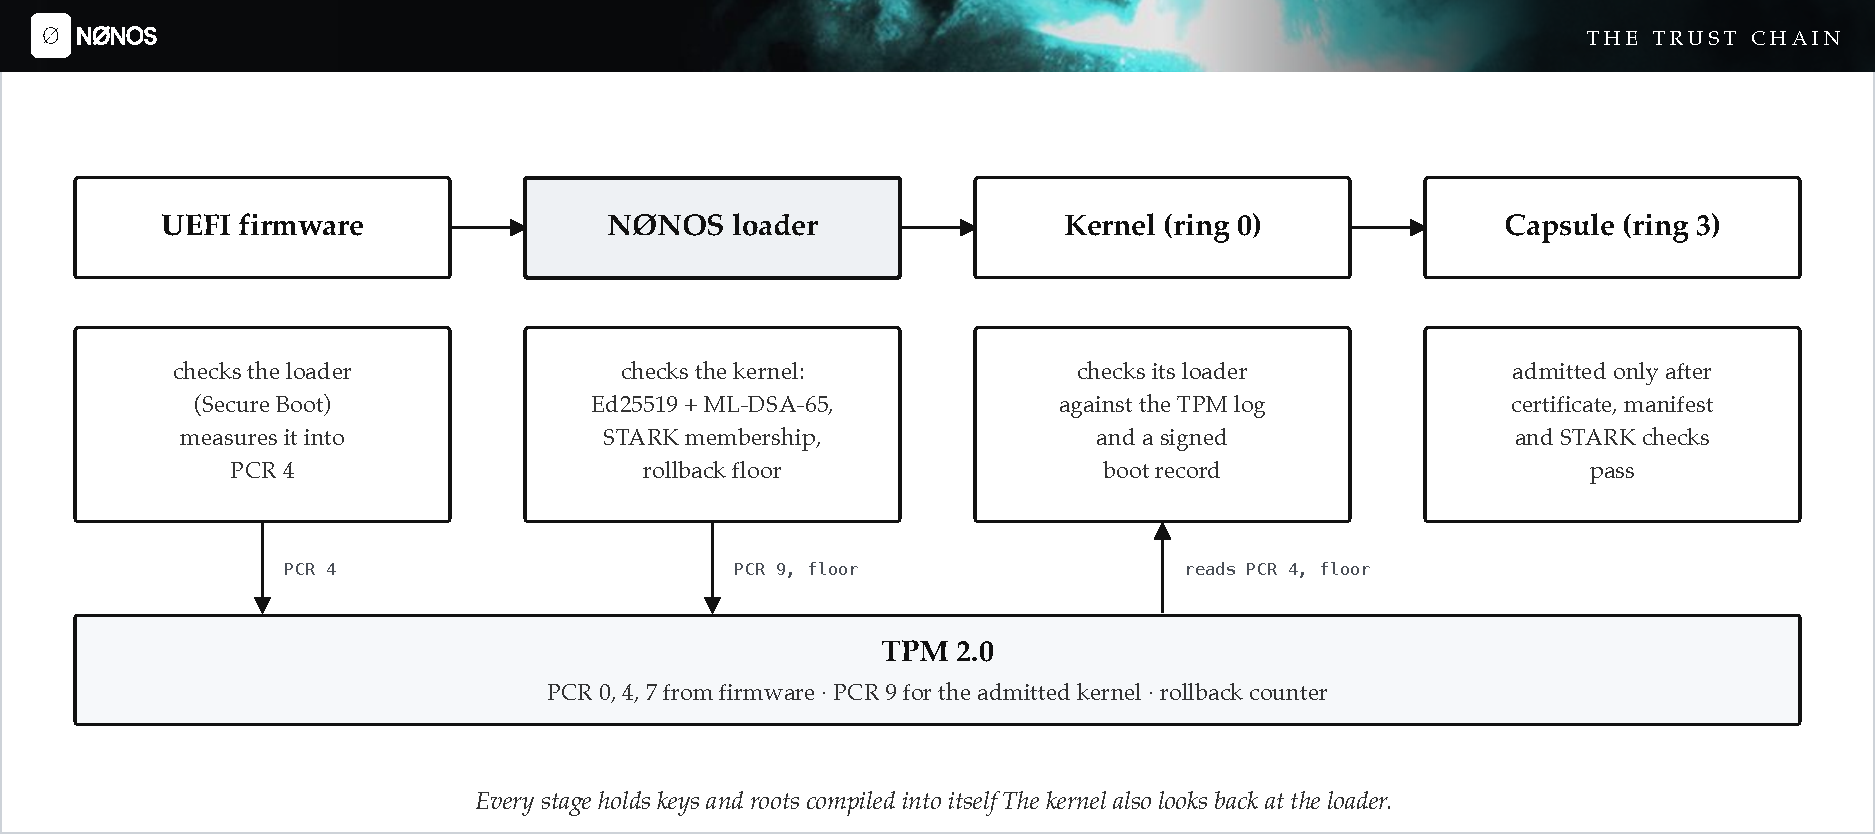
\includegraphics[width=0.84\textwidth]{figures/diagram-boot-chain.pdf}
\caption{The boot chain and the TPM registers each stage uses. Firmware measures the loader into PCR 4; the loader checks the kernel and extends PCR 9; the kernel checks the loader back against the TPM's event log and a signed boot-root record, then checks every capsule. Sources: \code{docs/security/boot-chain-and-signatures.md}, \code{docs/security/measured-boot-and-tpm.md}.}
\label{fig:boot}
\end{figure}

\subsection{The loader checks the kernel}

The kernel image carries a signature blob (\code{NKRSIG2}) with an Ed25519 signature and an ML-DSA-65 signature, each over the same 36-byte message: the BLAKE3 hash of the kernel ELF followed by the rollback index.\src{nonos-bootloader/tools/sign-kernel/src/message.rs:17-22} The public halves are compiled into the loader, and a production loader refuses to build without the ML-DSA-65 key.\src{nonos-bootloader/build.rs:135-216} The loader's pipeline runs the signature and rollback check, then \code{attest\_kernel} for the STARK trailer, then raises the TPM rollback floor, and only then hands over.\src{nonos-bootloader/src/entry/pipeline.rs:30-50} A kernel whose trailer fails is refused in every mode, development included.\src{nonos-bootloader/src/boot/attestation/kernel_gate.rs:34-60}

Figure~\ref{fig:bootshot} is the loader's screen on the sealed 0.9.3 image. It lists the ten steps, and step 7 is "Kernel STARK proof". The screen also says what was not there: Secure Boot off, no TPM, "TPM OFF: no TPM 2.0 measured boot". That run was under KVM, which gives the guest no TPM, so the chain's TPM half did not run in it.

\begin{figure}[t]
\centering
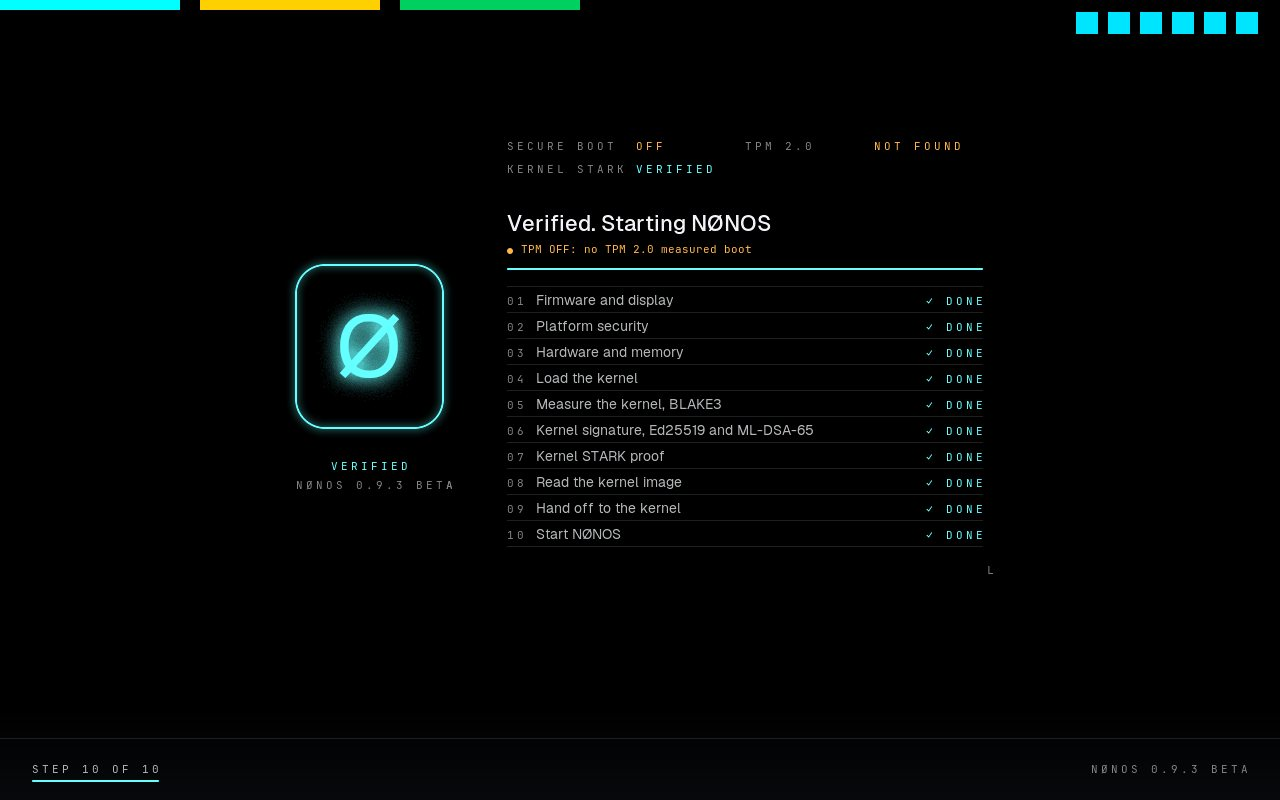
\includegraphics[width=0.55\textwidth]{figures/boot-verified.jpg}
\caption{The loader's screen on the sealed 0.9.3 image, under KVM, with no TPM and Secure Boot off, both shown in orange at the top. Steps 5 to 7 measure the kernel with BLAKE3, check the Ed25519 and ML-DSA-65 signatures, and check the kernel's STARK proof. This is one boot of one image on a virtual machine; it shows the kernel proof checked and says nothing about the TPM path or about a machine with Secure Boot on.}
\label{fig:bootshot}
\end{figure}

\subsection{The kernel checks its loader}

Before init, \code{check\_bootloader} replays the firmware's TCG event log, requires it to reproduce the live PCR~4, takes the last application the log names as the loader, and holds that Authenticode digest to a 104-byte boot-root record signed with an ECDSA P-256 device-policy key compiled into the kernel, and to the loader's own STARK slot.\note{\path{nonos-boot-measure/src/gate/verdict.rs:22-58}; \path{docs/security/boot-chain-and-signatures.md}, section "The kernel checks its loader".} No program starts if the check refuses or finds no evidence.\src{src/kernel_core/init/entry/loader_refusal.rs:27-48} Without a TPM or a log, the kernel falls back to hashing the loader file the loader handed it, and says so in its verdict. That check then rests on the loader's own word.\srcs{nonos-boot-measure/src/gate/verdict.rs:60-75}{src/security/boot/loader_check/run.rs:34-55}

\subsection{The kernel checks every capsule}

A capsule ships its ELF with a \nonos{} ID certificate signed by the trust anchor, a manifest signed by its publisher, and an attestation trailer. \code{preflight} runs \code{verify\_id\_cert}, \code{verify\_with\_publisher} and \code{attest\_gate} in that order. Certificates and manifests need one valid signature of each algorithm. The manifest check covers eight conditions, from the certificate hash to the declared endpoints.\srcs{src/kernel_core/process_spawn/capsule_spawn/runner/preflight.rs:36-76}{src/security/capsule_manifest/verify/mod.rs:37-62} Section~\ref{sec:capsules} goes through admission.

\subsection{The STARK gate and its statement}

Every gate checks one statement: under root $R$, the leaf built from context $C$ with kind $K$ is a slot of a 256-slot tree. The gate builds $C$ itself from what it is about to run and grant. For a capsule, $C$ is 48 bytes: the BLAKE3 hash of the ELF, the capability word (8 bytes) and the policy epoch (8 bytes). For a kernel or loader, $C$ is the measurement and the boot epoch.\src{nonos-attest-path/src/context.rs:23-40} The leaf is a Poseidon permutation over the Goldilocks field of a domain word, the digest of $C$ and the kind, so a capsule slot cannot open as a kernel.\src{nonos-attest-path/src/leaf.rs:51-71}

The gate checks the statement twice, once by folding the Merkle path in the trailer up to the root, and once by running \code{nox\_verify} on a transparent STARK proof of the same slot. It admits only when both pass, and the root is always the gate's own compiled-in or signed value, never the trailer's.\src{src/security/capsule_attest/path.rs:45-53} The proof system is hash-based, with a Fiat-Shamir transcript, no trusted setup and no pairing. A trailer carries at most 256~KiB of proof.\src{nonos-attest-path/src/v4/layout.rs:32}

Three trees exist: the capsule policy tree, checked by the kernel at every spawn; the kernel tree, checked by the loader; and the bootloader tree, whose root is signed into the boot-root record because it cannot live inside the loader it measures.\note{\path{docs/security/stark-attestation.md}, section "Three trees".} \code{nonos-stark-enroll} builds them on the enrolling host, checks every proof with the gates' own verifier before writing it, and records a transcript from which anyone can recompute the root.\src{nonos-stark-enroll/src/stark/prove.rs:28-67} Figure~\ref{fig:who} shows where proofs are made and where they are checked.

\begin{figure}[t]
\centering
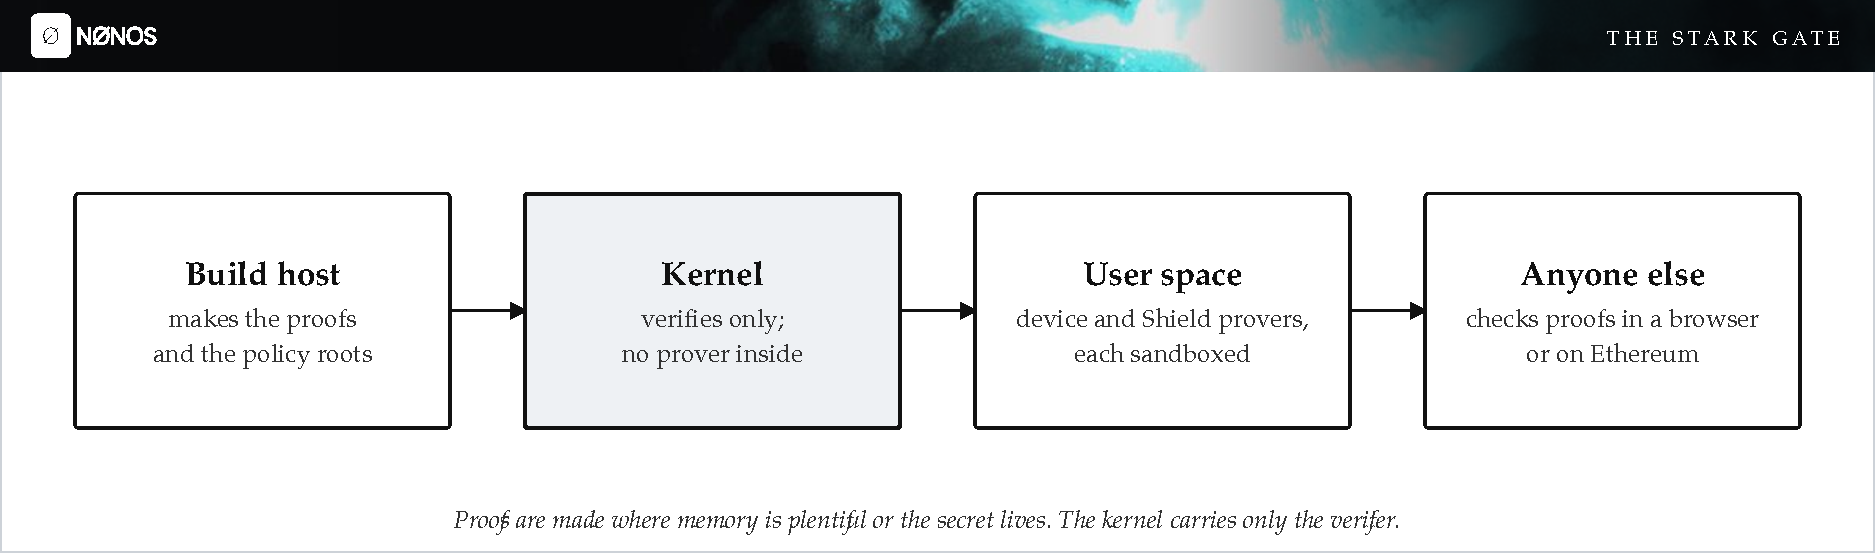
\includegraphics[width=0.84\textwidth]{figures/diagram-who-proves.pdf}
\caption{Who proves and who verifies. Proofs are made where memory is plentiful or where the secret lives. The kernel carries only the verifier. Sources: \code{README.md}, \code{docs/security/stark-attestation.md}.}
\label{fig:who}
\end{figure}

A trailer does not prove that the image is signed, that the capsule's code behaves, which slot it occupies (the path travels in the clear), or freshness by epoch. The path check rests on Poseidon's collision resistance and the proof's soundness on the STARKs repository, and no proof in the tree covers either.\note{\path{docs/security/stark-attestation.md}, section "What a trailer does not prove".} For this paper the middle item matters most. A STARK of membership is an identity statement. It says nothing about what a program does once it runs, and that is why Section~\ref{sec:box} exists.

\subsection{Measured boot, sealed keys and quotes}

The TPM never stores a \nonos{} key. The kernel asks it to derive keys under a PCR policy each time. The machine key, an HMAC under a primary key whose policy is the current value of PCRs 0, 4, 7 and 9, protects the data volume and sealed records, so the same disk in another machine, or the same machine in another boot state, gets another key.\srcs{src/security/tpm/machine_key/derive.rs:32-57}{src/security/tpm/machine_key/pcrs.rs:21-24} The device secret is derived under a policy the release signs over PCR~9, combined with this machine's PCRs 0, 4 and 7, so an approved kernel update keeps it while a firmware or loader change does not.\src{src/security/tpm/device_secret/derive.rs:33-54}

Two things are new in 0.9.3. A data volume formatted on a boot the release approved now has a random key, wrapped under a key the TPM gives only to a kernel the release approved. And an installed disk can be updated in place: from the moment the installed system prepares an update until the next boot, a one-boot handover record carries the key across a new bootloader. On QEMU with a software TPM, a prepared volume opened under an image with a changed bootloader through the handover, and then under that bootloader's own key. The window in which the handover record exists is a known weakness, listed in Section~\ref{sec:limits}.\note{\path{docs/release/0.9.3-what-is-new.md}, section "Update NØNOS (keep my data)"; \path{docs/release-evidence/0.9.3/s1-k1-update/README.md}.}

\code{MkAttestDoc} answers a 32-byte challenge with a TPM quote over PCRs 0, 1, 2 and 7. Because the attestation key is the same on every boot, a quote names the machine, so the kernel releases it only to a capsule that holds \code{AttestRead} and does not hold \code{Network}.\src{src/syscall/caps/checks/system.rs:40-52} The quote covers firmware state and not the PCRs \nonos{} itself extends; a design to quote the \nonos{} chain exists and is marked as design, with nothing landing before the 0.9.3 seal.\src{docs/design/k1-attest-doc-v4.md}

\subsection{The anonymous device proof}

\code{nonos-device-attest} proves, to a verifier who learns nothing else, four facts together: an approved bootloader started the machine, an approved kernel runs on it, the machine is an enrolled device, and a tag is this device's tag for the verifier's scope. The proof is made on the booted machine in a capsule that has no network bit and is the only one allowed \code{DeviceSecret}.\srcs{nonos-device-attest/README.md}{userland/capsule_prove/Capsule.mk:17-35} Its own README lists it as built and never run on a booted image, and we do not claim otherwise.\note{\path{nonos-device-attest/README.md}, section "What is not done".}
